%! TeX program = lualatex
\documentclass[a4paper]{article} 

% packages
\usepackage{microtype}      % Slightly tweak font spacing for aesthetics
\usepackage[english]{babel} % Language hyphenation and typographical rules
\usepackage[final, colorlinks = false, urlcolor = cyan]{hyperref} 
\usepackage{changepage}     % adjust margins on the fly

\usepackage{fontspec}
\setmainfont{EB Garamond}
\setmonofont[Scale=MatchLowercase]{Deja Vu Sans Mono}

\usepackage{minted}
\usepackage{xcolor}

\usepackage{pgfplots}
\pgfplotsset{width=\textwidth,compat=1.9}

\usepackage{caption}
\newenvironment{code}{\captionsetup{type=listing}}{}
% \captionsetup[listing]{font=small, skip=0pt}
% \setlength{\abovecaptionskip}{0pt}
% \setlength{\belowcaptionskip}{5pt}

\usepackage[yyyymmdd]{datetime}
\renewcommand{\dateseparator}{--}

\usepackage{titlesec}
% \titleformat{\section}{\LARGE\bfseries}{}{}{}[\titlerule]
% \titleformat{\subsection}{\Large\bfseries}{}{0em}{}
% \titlespacing{\subsection}{0em}{-0.7em}{0em}
%
% \titleformat{\subsubsection}{\large\bfseries}{}{0em}{$\bullet$ }
% \titlespacing{\subsubsection}{1em}{-0.7em}{0em}

% margins
\addtolength{\hoffset}{-2.25cm}
\addtolength{\textwidth}{4.5cm}
\addtolength{\voffset}{-3.25cm}
\addtolength{\textheight}{5cm}
\setlength{\parskip}{0pt}
\setlength{\parindent}{0in}
% \setcounter{secnumdepth}{0}

\begin{document}
\hrule \medskip
\begin{minipage}{0.295\textwidth} 
    \raggedright
    \footnotesize 
    Name: Andrew Hayes \\
    E-mail: \href{mailto://a.hayes18@universityofgalway.ie}{\texttt{a.hayes18@universityofgalway.ie}}  \hfill\\   
    ID: 21321503 \hfill
\end{minipage}
\begin{minipage}{0.4\textwidth} 
    \centering 
    \vspace{0.4em}
    \Large 
    \textbf{CT3531} \\ 
\end{minipage}
\begin{minipage}{0.295\textwidth} 
    \raggedleft
    \today
\end{minipage}
\medskip\hrule 
\begin{center}
    \normalsize
    Assignment 01: Expand the VLAN-Based Network
\end{center}
\hrule

\begin{figure}[H]
    \centering
    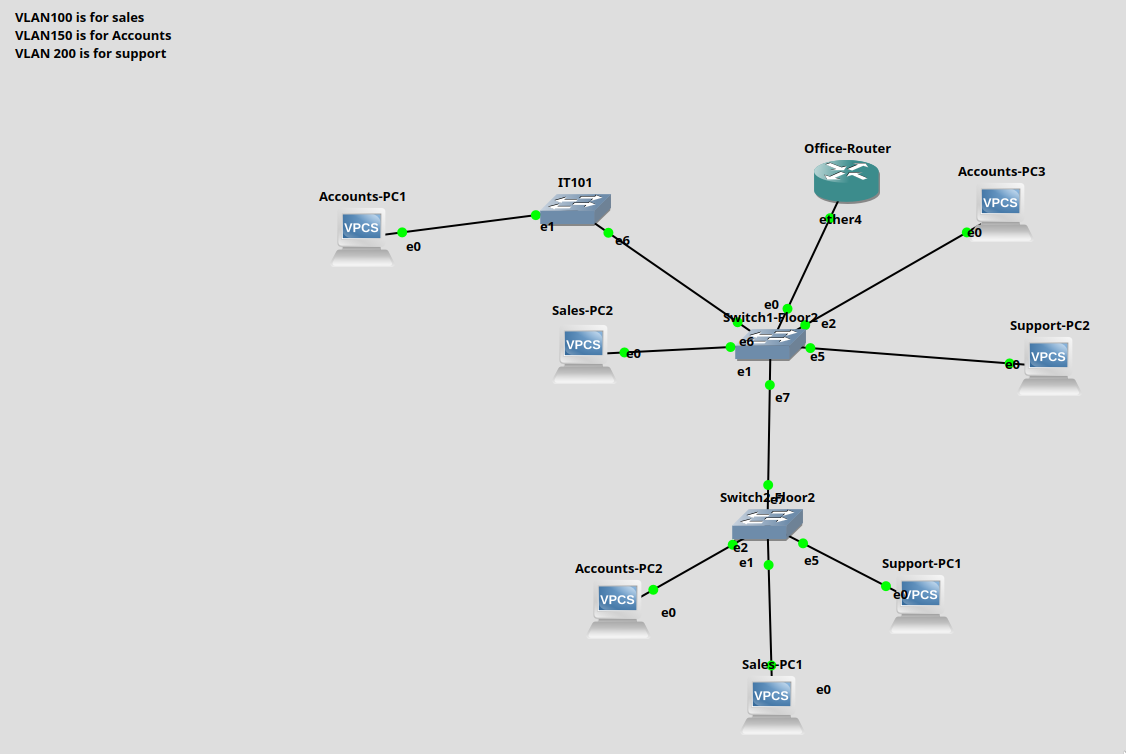
\includegraphics[width=0.8\textwidth]{./images/one.png}
    \caption{Network Topology}
\end{figure}

\begin{figure}[H]
    \centering
    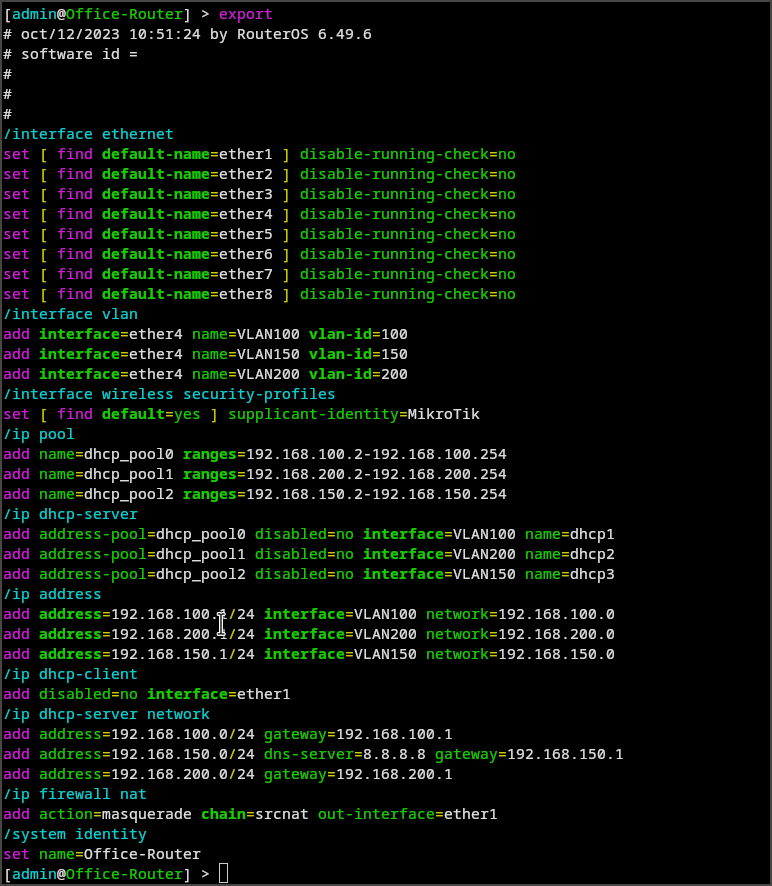
\includegraphics[width=0.635\textwidth]{./images/router_conf.png}
    \caption{Router Configuration}
\end{figure}

\begin{figure}[H]
    \centering
    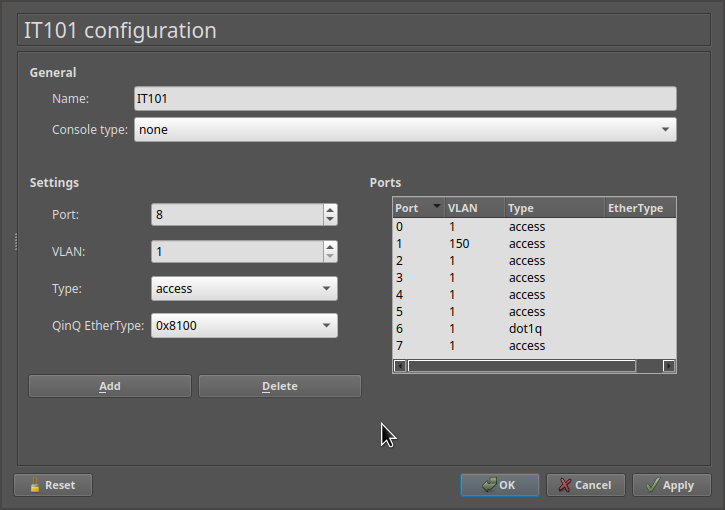
\includegraphics[width=0.6\textwidth]{./images/switch_conf.png}
    \caption{Configuration of the New IT101 Switch}
\end{figure}


\begin{figure}[H]
    \centering
    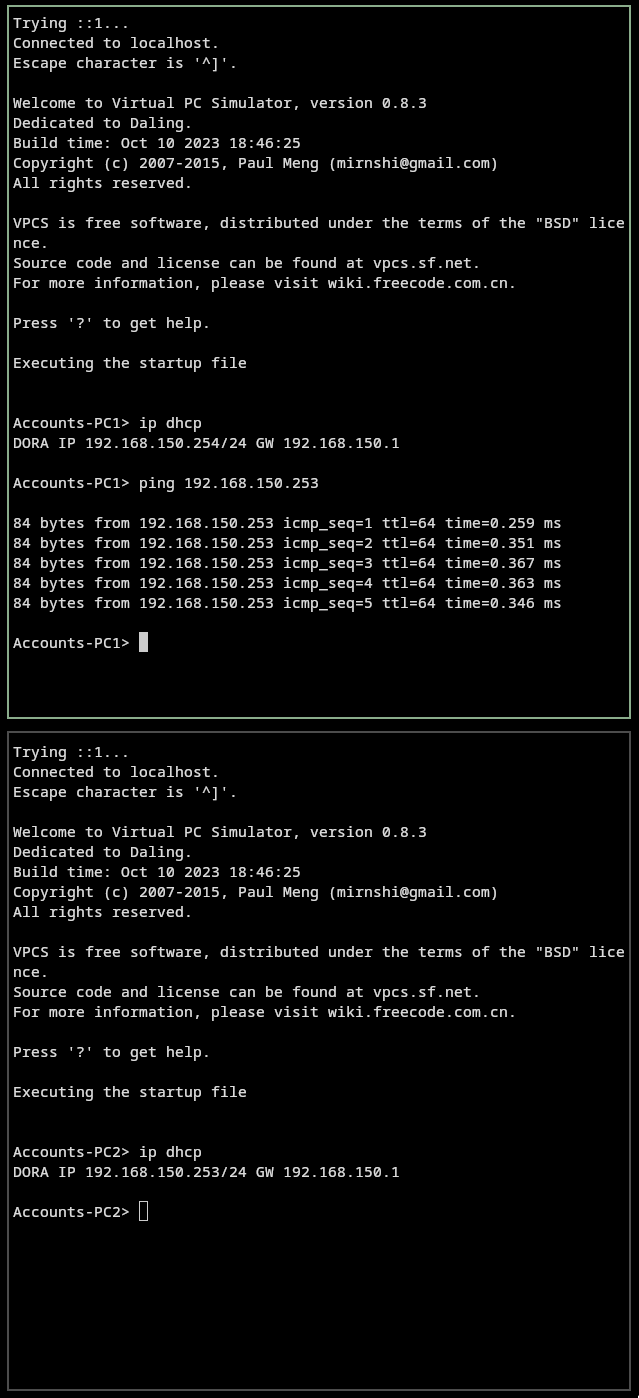
\includegraphics[width=0.45\textwidth]{./images/five.png}
    \caption{Verifying that The New VPC Devices in the Accounts VLAN Can Ping Each Other}
\end{figure}

\begin{figure}[H]
    \centering
    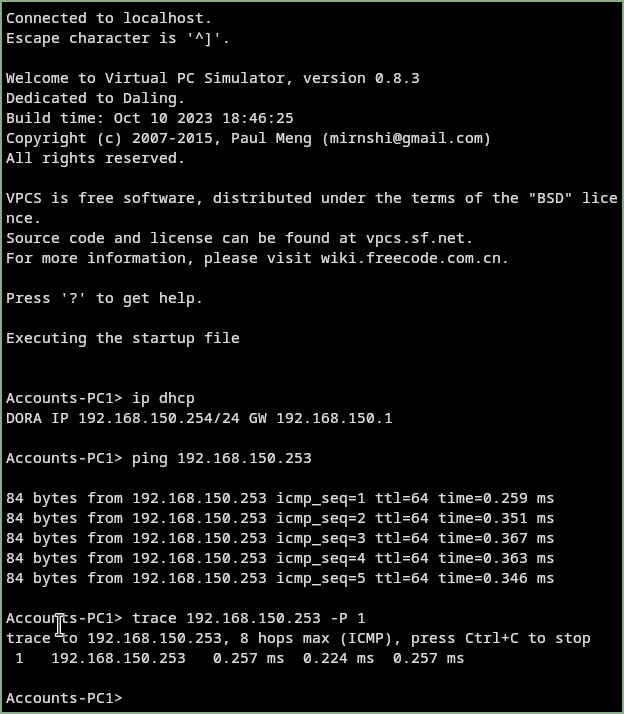
\includegraphics[width=0.5\textwidth]{./images/six.png}
    \caption{Running a Trace from a VPC to Another VPC in the Same VLAN (Same VPCs as in Above Figure)}
\end{figure}

When we run a trace from Accounts-PC1 to Accounts-PC2 (which are both on VLAN150), we can see that it only takes one hop to get from Accounts-PC1 to Accounts-PC2. 
Because these devices are in the same VLAN, they do not need to go through the router to address each other, and can reach other directly.
When devices share a VLAN, they can communicate directly at the Data Link Layer.

\begin{figure}[H]
    \centering
    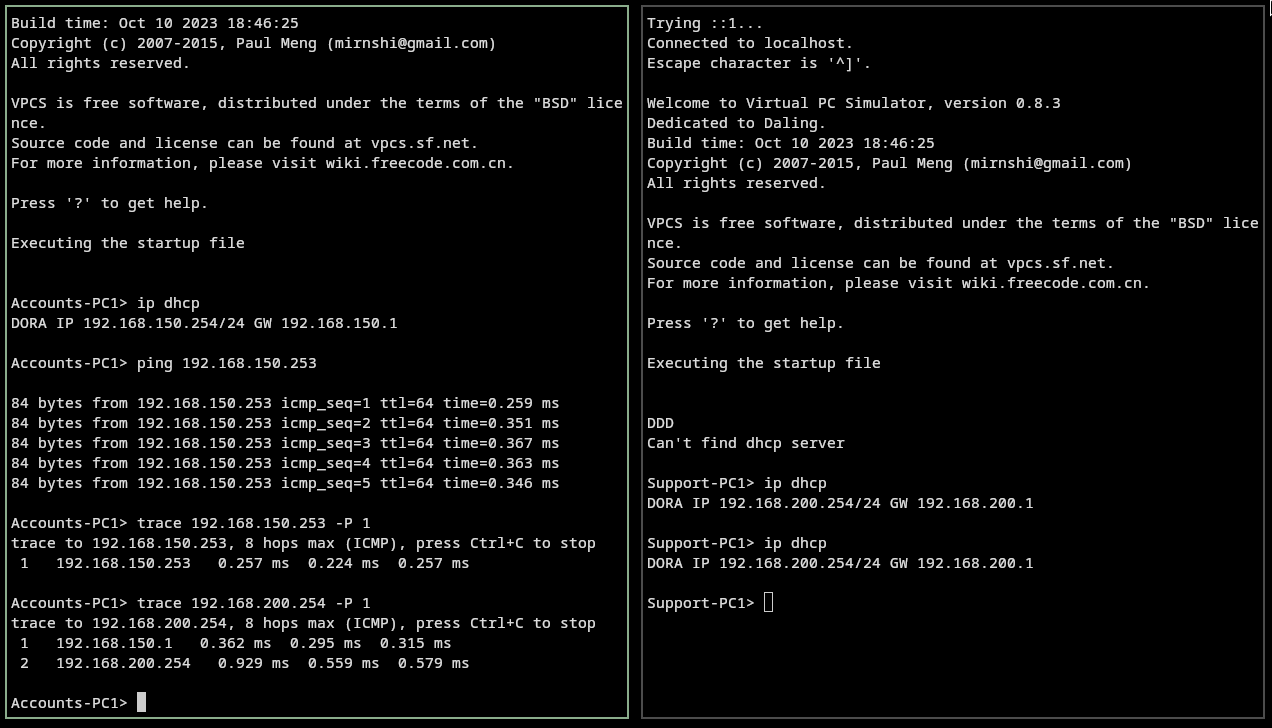
\includegraphics[width=0.9\textwidth]{./images/seven.png}
    \caption{Running a Trace from a VPC to Another VPC in Different VLANs}
\end{figure}

When we run a trace from Accounts-PC1 to Support-PC1 (which are on different VLANs), we can see that it takes two hops to get from Accounts-PC1 to Support-PC1. 
Communication between separate VLANs requires routing, and therefore communicating between two devices on two different VLANs requires that the packets go through a
router. 
The first IP in the trace is that of the router: \verb|192.168.150.1| (or rather the IP of the gateway of VLAN150 on the router).
The second IP in the trace is that of Support-PC1: \verb|192.168.200.254|.

\begin{figure}[H]
    \centering
    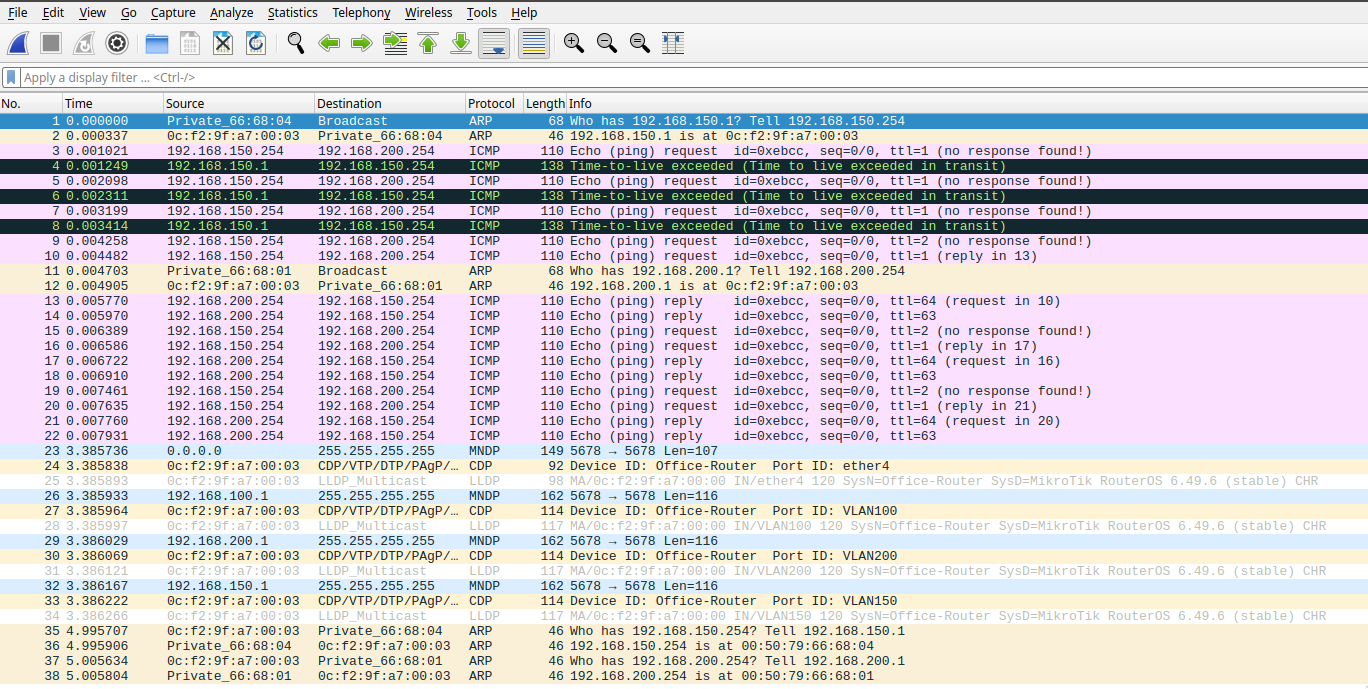
\includegraphics[width=\textwidth]{./images/eight.png}
    \caption{Packet Capture on the Link Connecting the Switch \& the Router During a Ping between VPCs on Different VLANs}
\end{figure}

The general outline of what happened in this packet capture is as follows:
\begin{enumerate}
    \item   An ICMP ping is sent from Accounts-PC1 (which is on VLAN150) to Support-PC1 (which is on VLAN200).
            Ethernet frames that travel between VLANs need a tag that identifies the VLAN as per the 802.1Q protocol.
            However, the 802.1Q is not added by the VPC sending the ping; instead, the tag is added by the first switch that the frame passes through, in this case 
            the IT101 switch.
            The IT101 switch will have encapsulated the packet with an 802.1Q header and added the VLAN information, including the priority bits, the VLAN ID of the 
            VLAN to which the packet belongs, \& the Canonical Format Indicator which indicates the canonical format of the MAC address.
            Therefore, by the time the packet reaches the Switch1-Floor2 switch, the VLAN tag has already been added to the frame. 

    \item   The Switch1-Floor2 switch then forwards the encapsulated packet which now contains the 802.1Q header to the Office-Router router.
            This can be seen in the first ICMP packet that we captured going from \verb|192.168.150.254| (Accounts-PC1) to \verb|192.168.200.254| (Support-PC1): 
            \begin{figure}[H]
                \centering
                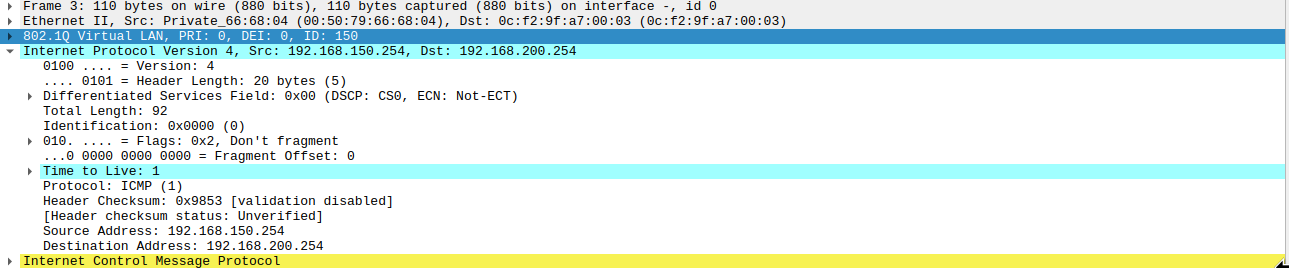
\includegraphics[width=0.9\textwidth]{./images/dot1q_tag.png}
                \caption{ICMP Packet Containing the 802.1Q Tag}
            \end{figure}

    \item   We can tell what links require an 802.1Q header by checking whether they are trunks or access links: trunks expect packets to have an 802.1Q header so 
            that the switches or routers that they are linking can know which VLAN they belong to.
            Access links do not expect an 802.1Q header, as the ports which access links join are specified to belong to a certain VLAN when the switch is configured.
            Therefore every packet traversing one of the trunk links, i.e. IT101 {\leftrightarrow} Switch1-Floor2, Switch1-Floor2 {\leftrightarrow} Office-Router,
            \& Switch1-Floor2 {\leftrightarrow} Switch2-Floor2, requires a 802.1Q header.   
            The last switch (Switch2-Floor2) before the destination VPC (Support-PC1) will remove the 802.1Q header, extracting the original ICMP echo request packet, and send it
            down the access link to Support-PC1.

    \item   The router is needed to facilitate the inter-VLAN communication;
            although, in purely physical terms, data could be transferred via the switches from Accounts-PC1 to Support-PC1 without having to go to the router, the 
            router is needed to facilitate inter-VLAN communication over IP, as the VLANs have separate broadcast domains and the individual VPCs do not know which 
            VLAN they belong to, if any.
            The router forwards the packets to the switch Switch1-Floor2, which passes them to Switch2-Floor2.
    
    \item   When the ICMP packets reach Switch2-Floor2, the 802.1Q header is stripped from them, as they have now traversed the last trunk link that they need to 
            and are now going to pass over an access port to Support-PC1.
            Since we are capturing the packets over the trunk link between a Switch1-Floor2 \& Office-Router, we will never see a packet without an 802.1Q header, 
            although they are in use for this ping.

    \item   When the echo request reaches Support-PC1, it send back an echo reply via Switch2-Floor2. 
            The 802.1Q header will be added at Switch2-Floor2, and the process will repeat to route the packet across the trunks to the router, and then to the 
            IT101 switch, where the 802.1Q header will be stripped and the packet forwarded back to Accounts-PC1, completing the ping.
\end{enumerate}

\end{document}
